\textbf{COLUNI 2025 -- Questão 12}\par\medskip Um terreno tem o formato do triângulo $ABC$ apresentado na figura abaixo. O proprietário deste terreno decide vender uma parte, dividindo o mesmo em duas regiões $R_1$ e $R_2$, sendo $R_1$ representada pelo triângulo $ADE$ e $R_2$ pelo trapézio $BCDE$. Sabe-se que o segmento de reta $\overline{DE}$ é paralelo ao lado $\overline{BC}$, $\overline{AB}=12\,\text{km}$, $\overline{AE}=10\,\text{km}$, $\overline{EC}=6\,\text{km}$, $\overline{DE}=3\,\text{km}$ e $\overline{DB}=x\,\text{km}$.

% COLUNI-AUTO-FIGURES-BEGIN
\begin{figure}[htbp]
\centering
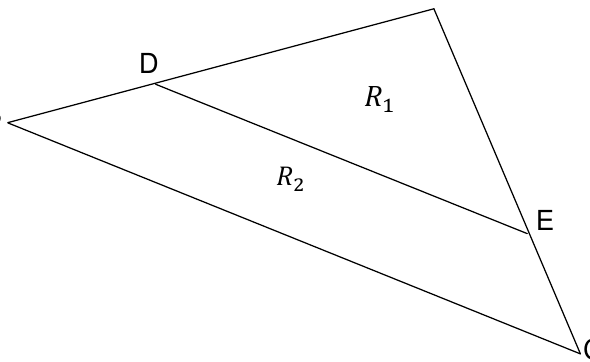
\includegraphics[width=0.75\linewidth]{static/simulados/coluni/figuras/2025/questao-12/figura-1.png}
\end{figure}
% COLUNI-AUTO-FIGURES-END

É CORRETO afirmar que o perímetro da região $R_1$ é dado por:
\begin{enumerate}
\item 21 Km.
\item 20 Km.
\item 21,5 Km.
\item 20,5 Km.
\end{enumerate}
